\cohead{\Large\textbf{Monotonie}}
\fakesubsection{Monotonie}
Die Begriffe positive/negative Steigung bzw. steigende/fallende Funktion haben wir bereits intuitiv verwendet. Jetzt wollen wir diese mathematisch definieren.
\begin{tcolorbox}
	Monoton wachsende Funktionen:\\
	\textcolor{loestc}{Eine Funktion \(f(x)\) ist monoton wachsend, wenn die Funktionswerte mit steigenden x-Werten größer werden.\\
	}
\end{tcolorbox}
\begin{minipage}{\textwidth}
	\begin{minipage}{0.6\textwidth}
		Beispiel: \(f(x)=\frac{1}{10}x^3\)\\
		\textcolor{loes}{Aus \(x_1\leq x_2\) folgt \(f(x_1 )\leq f(x_2)\)\\
			Diese Funktion ist auf ganz \(\R\) monoton wachsend.\\
			Beim Zeichnen des Schaubilds der Funktion muss man mit dem Stift immer weiter nach oben gehen.}\\ \\
	\end{minipage}
	\begin{minipage}{0.39\textwidth}
		\centering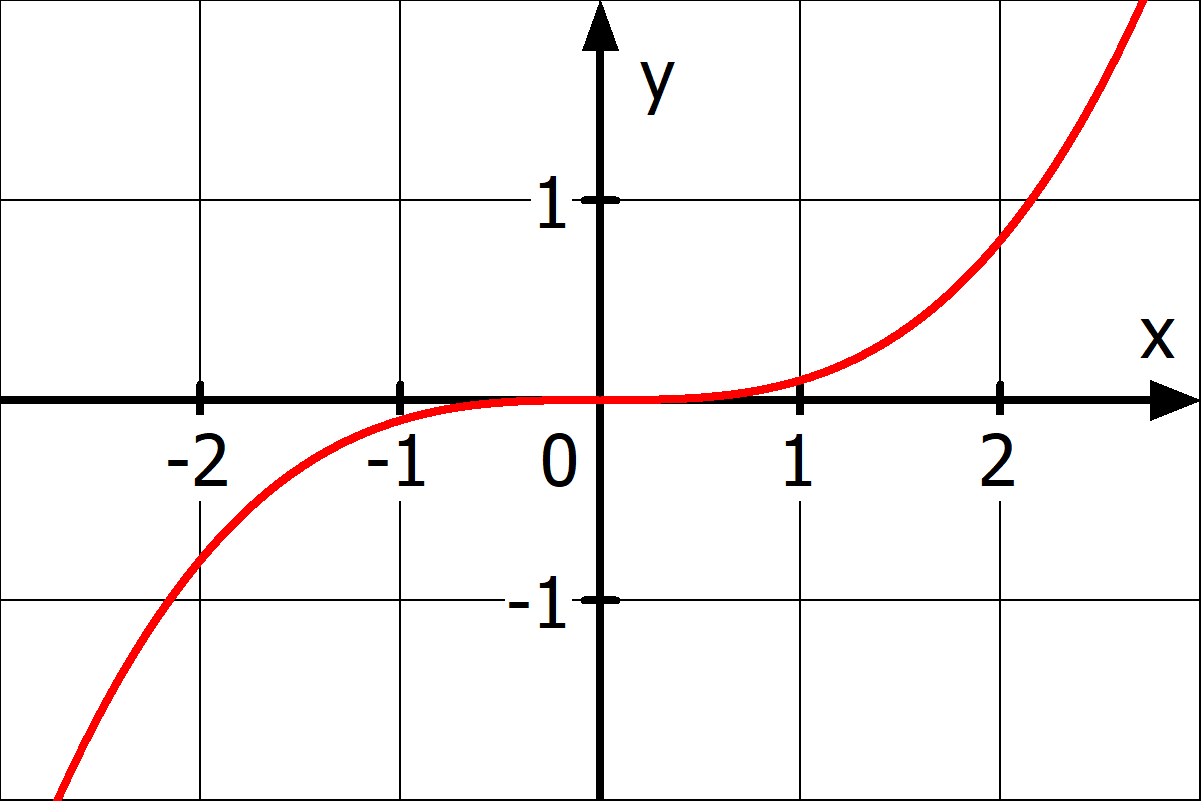
\includegraphics[width=.9\textwidth]{\ableitung/pics/monotonieBsp1.png}\\
	\end{minipage}
\end{minipage}\\

\begin{tcolorbox}
	Monoton fallende Funktionen:\\
	\textcolor{loestc}{Eine Funktion \(f(x)\) ist monoton fallend, wenn die Funktionswerte mit steigenden x-Werten kleiner werden.\\
	}
\end{tcolorbox}
\begin{minipage}{\textwidth}
	\begin{minipage}{0.6\textwidth}
		Beispiel: \(f(x)=e^{-x}-1\)\\
		\textcolor{loes}{Aus \(x_1\leq x_2\) folgt \(f(x_1 )\geq f(x_2)\)\\
			Diese Funktion ist auf ganz \(\R\) monoton fallend.\\
			Beim Zeichnen des Schaubilds der Funktion muss man mit dem Stift immer weiter nach unten gehen.}\\ \\
	\end{minipage}
	\begin{minipage}{0.39\textwidth}
		\centering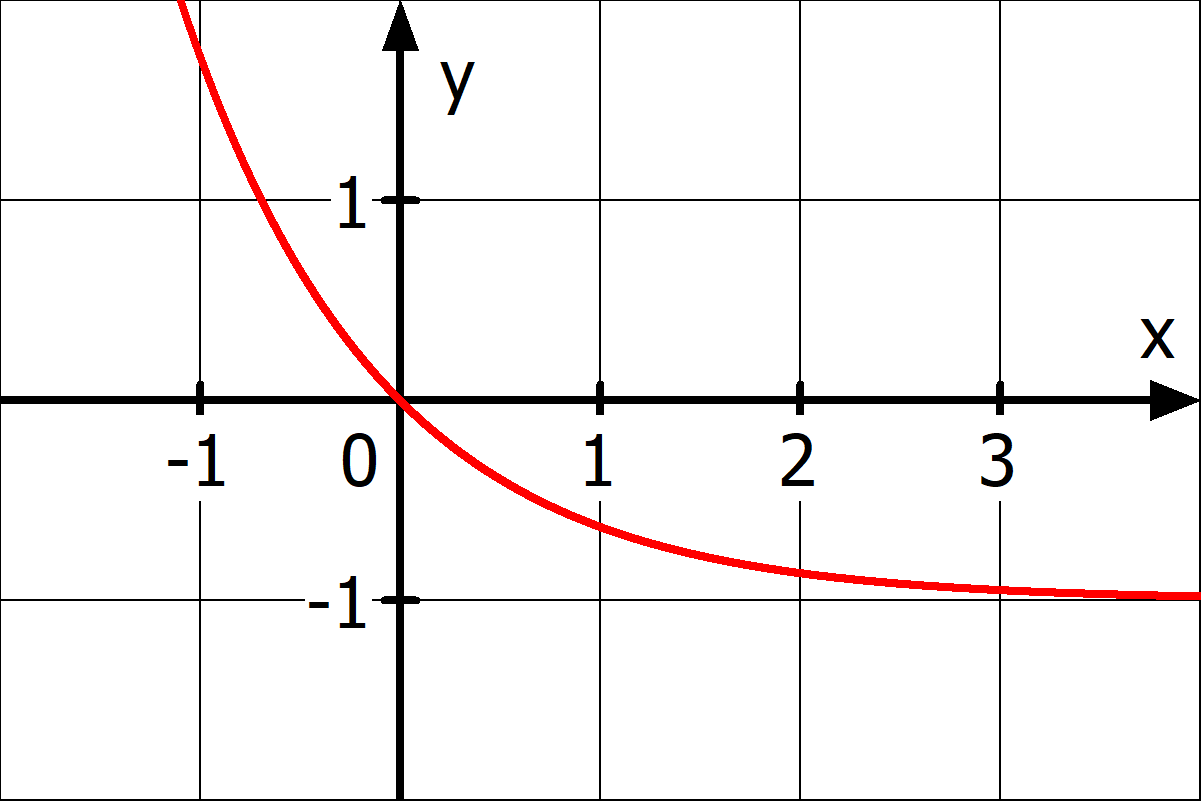
\includegraphics[width=.9\textwidth]{\ableitung/pics/monotonieBsp2.png}\\
	\end{minipage}
\end{minipage}\\ \\ \\
\begin{minipage}{\textwidth}
	\begin{minipage}{0.39\textwidth}
		\centering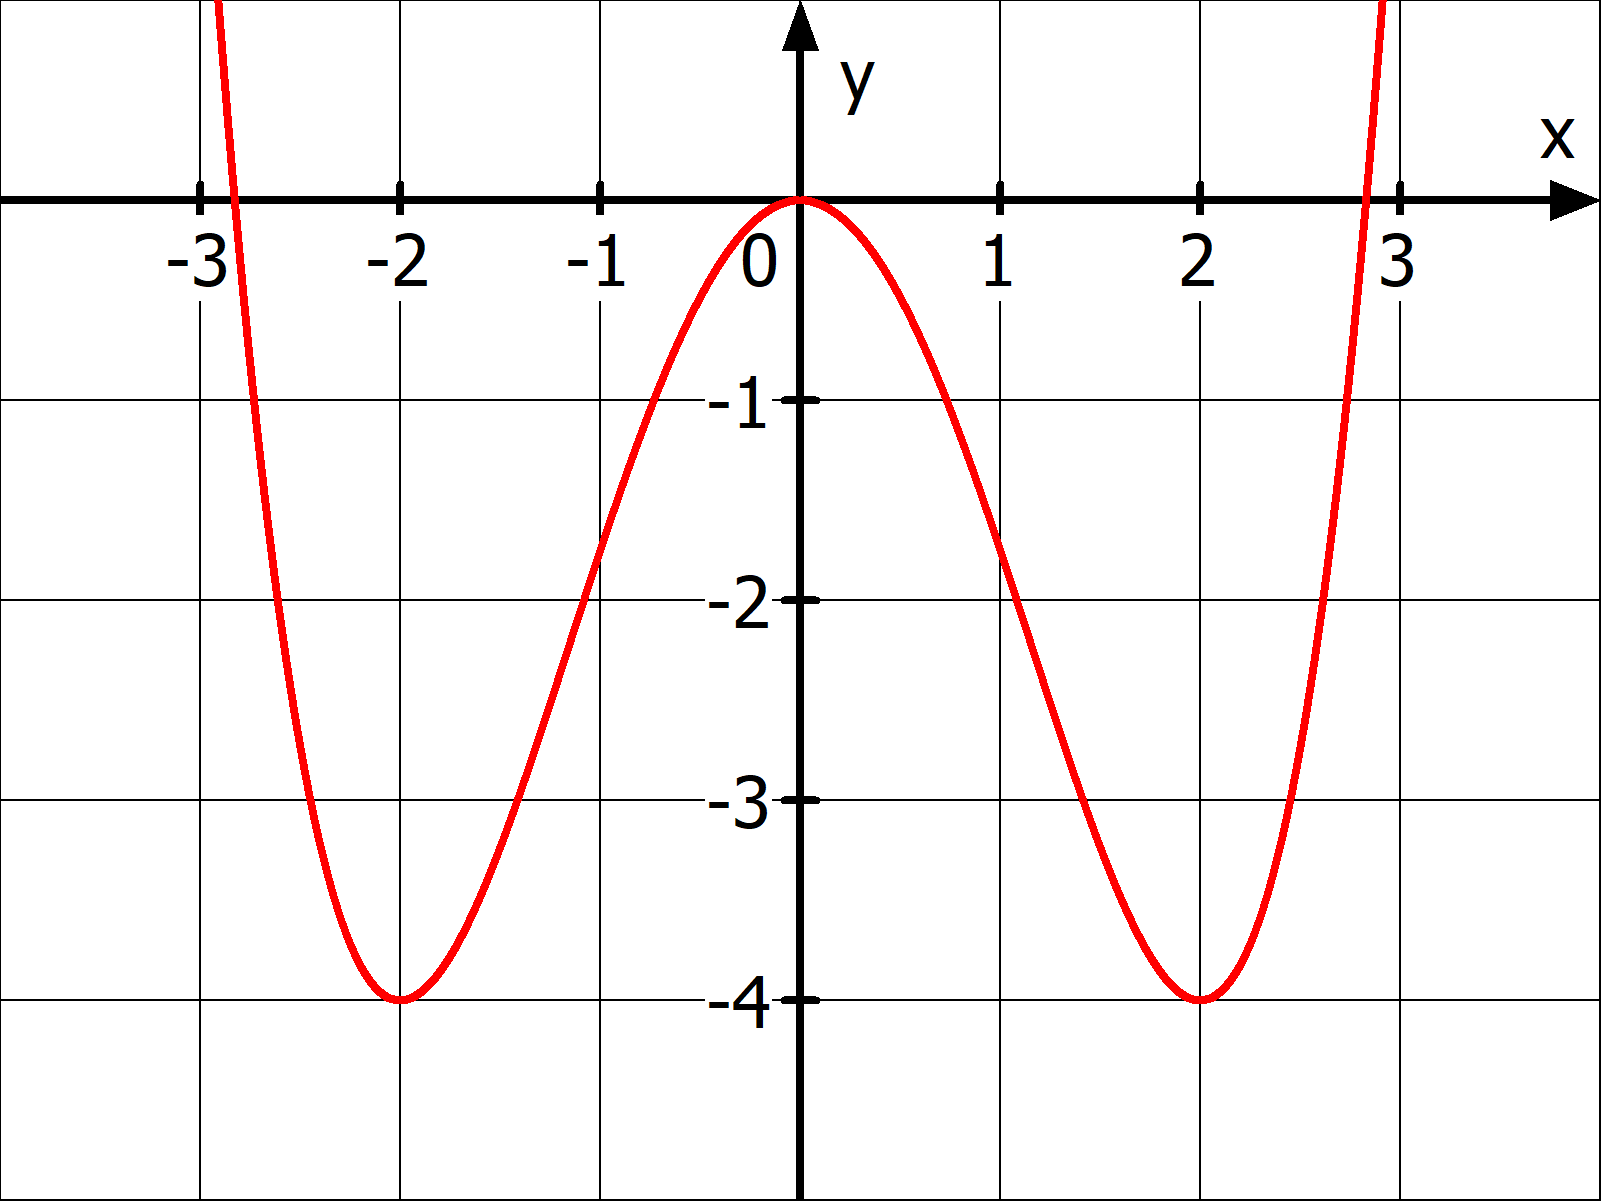
\includegraphics[width=.9\textwidth]{\ableitung/pics/monotonieBsp3.png}\\
	\end{minipage}
	\begin{minipage}{0.6\textwidth}
		Monotonie kann auch für Intervalle definiert werden:\\
		Die Funktion \(f(x)=\frac{1}{4}x^4-2x^2\) hat folgende Monotonieintervalle:\\
		\textcolor{loes}{
			Auf den Intervallen \(]-\infty,\ -2]\) und \([0,\ 2]\) ist die Funktion monoton fallend.\\
			Auf den Intervallen \([-2,\ 0]\) und \([2,\ \infty[\) ist die Funktion monoton steigend.}\\
	\end{minipage}
\end{minipage}\\
\textcolor{loes}{Hinweis: Wir unterscheiden nicht zwischen Monotonie und strenger Monotonie}
\newpage
%%%%%%%%%%%%%%%%%%%%%%%%%%%%%%%%%%%%%%%%%%%%%%%%%%%%%%%%%%%%%%%%%%%%%%%%%%%%%%%%%%%%%%%%%%%%%%%%%%%%%%%
\begin{Exercise}[title={\raggedright Bestimme die Monotonieintervalle.}, label=monotonieA1]\\
	\begin{minipage}{\textwidth}
		\begin{minipage}{0.33\textwidth}
			\centering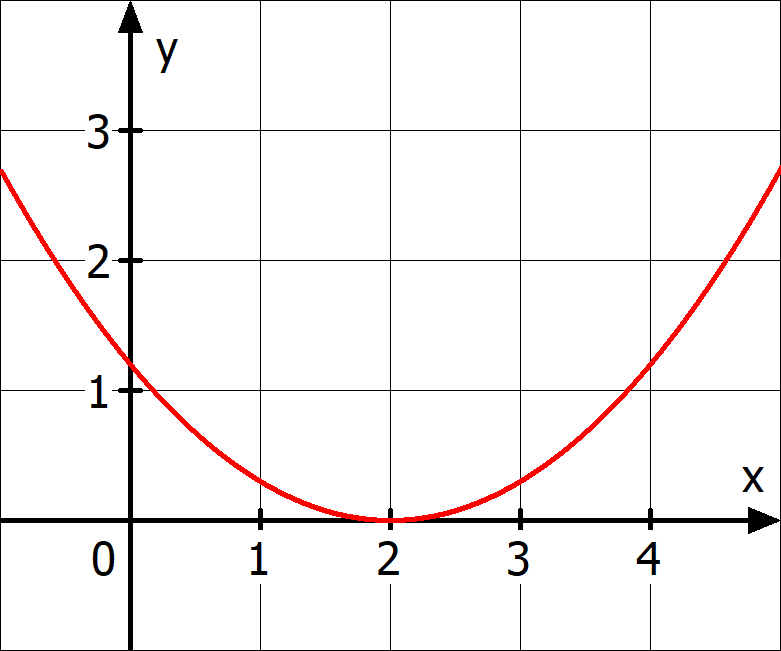
\includegraphics[width=.95\textwidth]{\ableitung/pics/monotonieIntervalle1.png}\\
		\end{minipage}
		\begin{minipage}{0.33\textwidth}
			\centering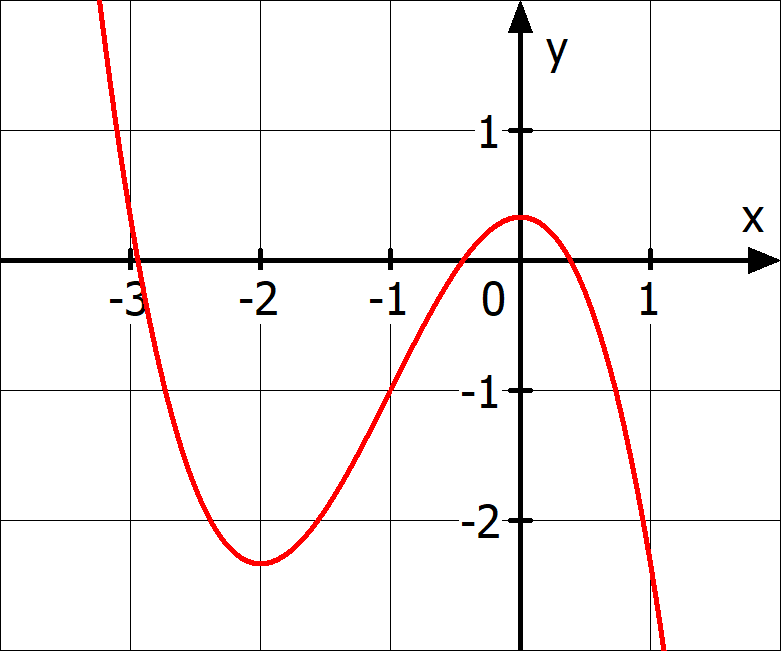
\includegraphics[width=.95\textwidth]{\ableitung/pics/monotonieIntervalle2.png}\\
		\end{minipage}
		\begin{minipage}{0.33\textwidth}
			\centering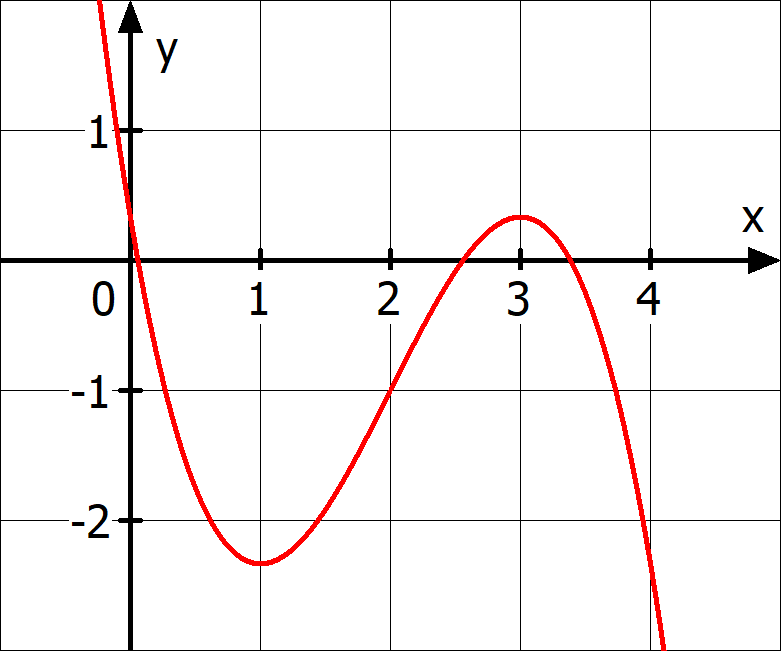
\includegraphics[width=.95\textwidth]{\ableitung/pics/monotonieIntervalle3.png}\\
		\end{minipage}\\ \\ \\
		\begin{minipage}{0.33\textwidth}
			\centering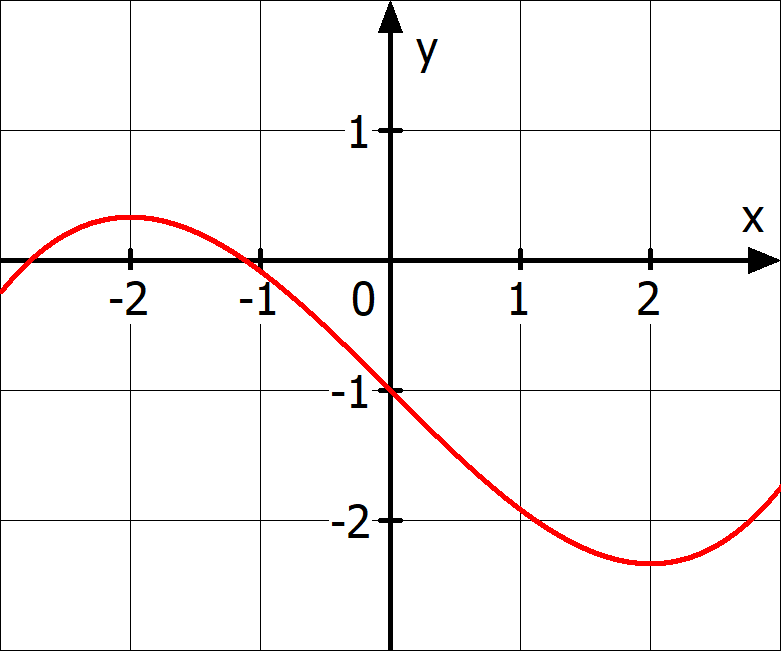
\includegraphics[width=.95\textwidth]{\ableitung/pics/monotonieIntervalle4.png}\\
		\end{minipage}
		\begin{minipage}{0.33\textwidth}
			\centering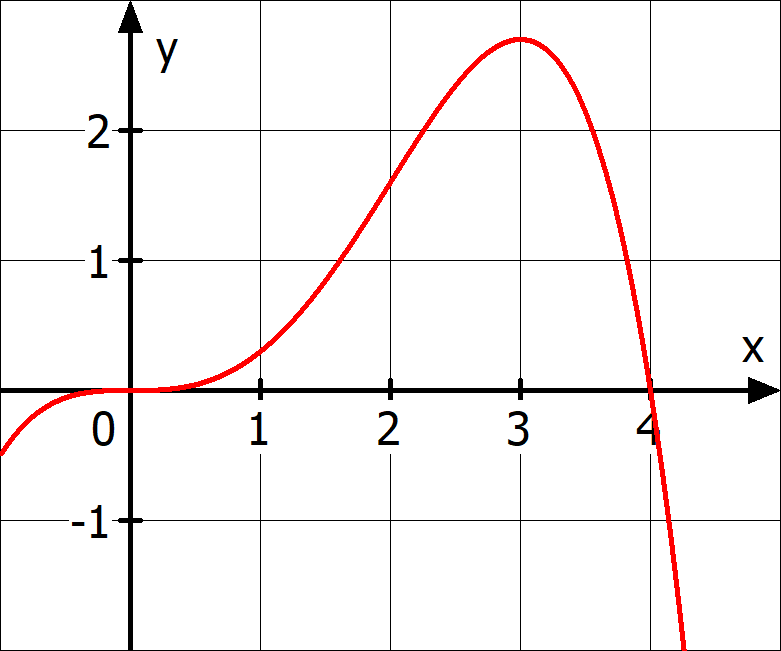
\includegraphics[width=.95\textwidth]{\ableitung/pics/monotonieIntervalle5.png}\\
		\end{minipage}
		\begin{minipage}{0.33\textwidth}
			\centering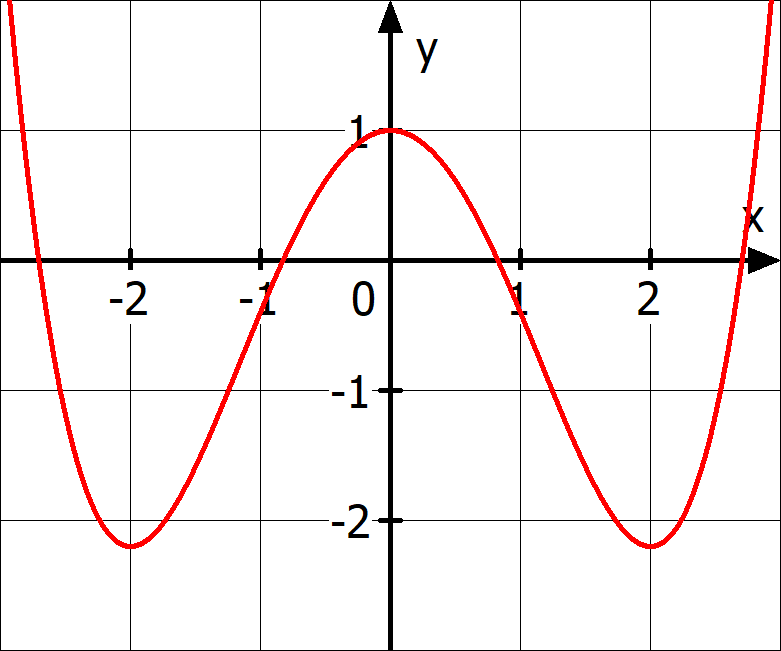
\includegraphics[width=.95\textwidth]{\ableitung/pics/monotonieIntervalle6.png}\\
		\end{minipage}\\ \\ \\
		\begin{minipage}{0.33\textwidth}
			\centering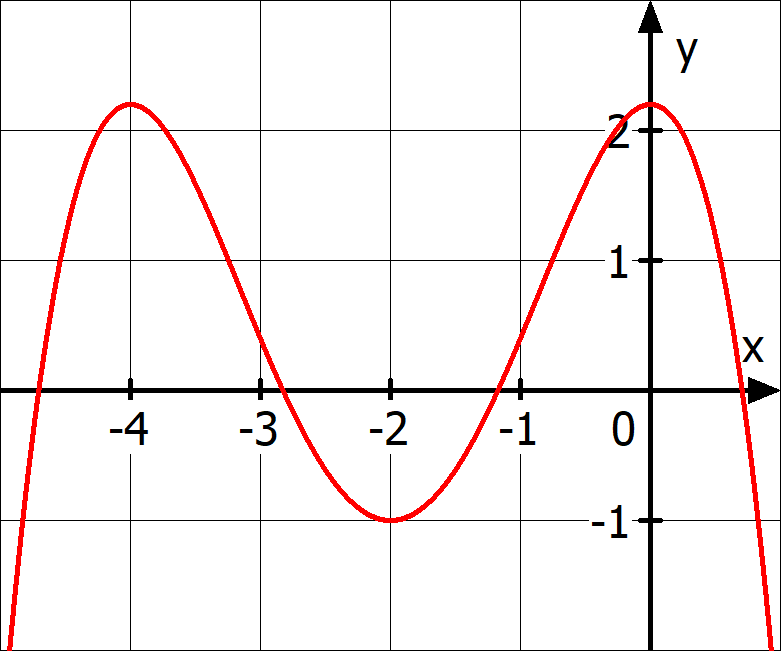
\includegraphics[width=.95\textwidth]{\ableitung/pics/monotonieIntervalle7.png}\\
		\end{minipage}
		\begin{minipage}{0.33\textwidth}
			\centering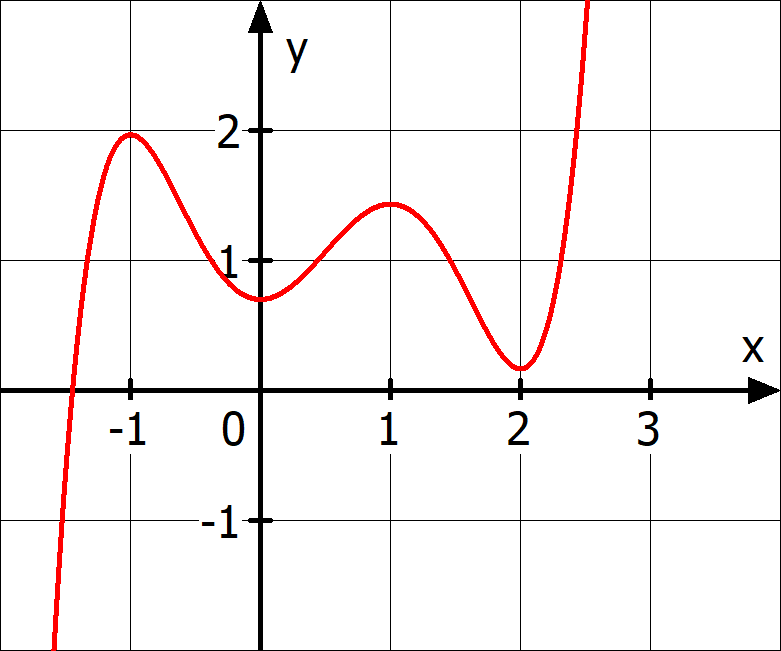
\includegraphics[width=.95\textwidth]{\ableitung/pics/monotonieIntervalle8.png}\\
		\end{minipage}
		\begin{minipage}{0.33\textwidth}
			\centering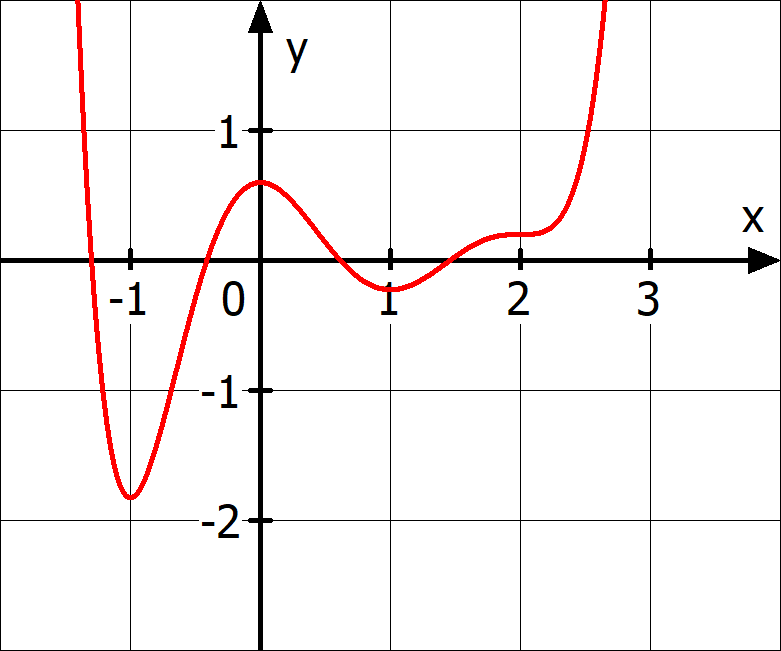
\includegraphics[width=.95\textwidth]{\ableitung/pics/monotonieIntervalle9.png}\\
		\end{minipage}\\ \\ \\
	\end{minipage}
\end{Exercise}
%%%%%%%%%%%%%%%%%%%%%%%%%%%%%%%%%%%%%%%%%
\begin{Answer}[ref=monotonieA1]\\
	\begin{tabular}{p{.3\textwidth}|p{.3\textwidth}|p{.3\textwidth}}
		\hline
		Monoton fallend auf\newline \(]-\infty;2]\)\newline
		Monoton steigend auf\newline \([2;\infty[\)
		&
		Monoton fallend auf\newline \(]-\infty;-2]\) und \([0;\infty[\)\newline
		Monoton steigend auf\newline \([-2;0]\)
		&
		Monoton fallend auf\newline \(]-\infty;1]\) und \([3;\infty[\)\newline
		Monoton steigend auf\newline \([1;3]\)
		\\
		\hline
		Monoton fallend auf\newline \([-2;2]\)\newline
		Monoton steigend auf\newline \(]-\infty;-2]\) und \([2;\infty[\)
		&
		Monoton fallend auf\newline \([3;\infty[\)\newline
		Monoton steigend auf\newline \(]-\infty;3]\)
		&
		Monoton fallend auf\newline \(]-\infty;-2]\) und \([1;2]\)\newline
		Monoton steigend auf\newline \([-2;0]\) und \([2;\infty[\)
		\\
		\hline
		Monoton fallend auf\newline \([-4;-2]\) und \([0;\infty[\)\newline
		Monoton steigend auf\newline \(]-\infty;-4]\) und \([-2;0]\)
		&
		Monoton fallend auf\newline \([-1;0]\) und \([1;2]\)\newline
		Monoton steigend auf\newline \(]-\infty;-1]\), \([0;1]\) und \([1;\infty[\)
		&
		Monoton fallend auf\newline \(]-\infty;-1]\) und \([0;1]\)\newline
		Monoton steigend auf\newline \([-1;0]\) und \([1;\infty[\)
		\\
		\hline
	\end{tabular}
\end{Answer}